% Drawing 127/01-3 -- folder 127, batch 01, archive page 10 (PDF page 11).
% Transcription: croquis, sous « EGA IV 9 » ; points $x_0$, $x'_0$ sur $X'$, $x$, $x'$ sur $X$, $y$, $y'$ sur $Y$, $y_0$, $y'_0$ sous $Y'$ ; à côté un second croquis semblable, où $X'$ et $Y'$ sont reliés à $X$, $Y$ par des traits obliques, avec $Y''$ \uncertain{et} $y''_0$, $y_0$ ; les directions des traits sans flèche ne sont pas marquées
% Kind: two sketches of base changes with points. Method 2 (schematic redraw from the facsimile). Status: ok.
% Notes: Left sketch, under "EGA IV 9": X' (with x_0, x'_0 to its left), X (with x, x'), Y' (with y_0, y'_0 below), Y (with y, y'); X' - X, X - Y, Y' - Y; between Y' and X' two strokes, a plain one and an arrow up (Y' -> X'); the arrow Y' -> X. Right sketch, fainter: X' (x_0, x'_0 beside it), X, Y'', Y; X' - X and Y'' - Y oblique, X - Y, X' - Y'' with a faint arrow up beside it, and a dashed oblique from X towards Y''; y''_0, y_0 below. Nodes placed once, every stroke on the line between the same two node points; directions of plain strokes not marked, as in the transcription. Still differs: in the right sketch the labels beside X' are small and overinked (read x_0, x'_0 as in the left sketch) and the x right of X is cut by the crop edge. Redrawn 2026-11-09 (issue 128): to check again. Question settled by a machine pass on the facsimile, 2026-11-12 (page): the two small labels left of X' in the right sketch read x_0 and x'_0 on a 300 dpi crop, as in the left sketch and as drawn. Not checked by a reader. 2026-11-14, Claude Opus 5.5, overlay check (issue 147): rasterised from its own coordinates over the 400 dpi colour scan on a unit grid, corrected and measured; not compiled (no TeX in the session). Changed: in the left sketch the strokes X' - X, X - Y, Y' - Y and Y' - X' and the two arrows moved 0.7 to 1.5 units onto their ink (the plain stroke Y' - X' and the arrow beside it lay to the left of the page's); « EGA IV 9 » centred on its writing; in the right sketch the dashed oblique now runs from beside X to above Y'' along its dashes, the stroke Y'' - Y moved onto its ink, and the x written right of X is set (it lies inside the crop). Every stroke and label lies on its ink to within about 1 unit; the faint arrow beside X' - Y'' stays where it was drawn, on its faint stroke. Status set to ok.
% Coordinates: 1 unit = 1 mm = 1/100 of the crop width (bbox in page fractions: [0.07, 0.62, 0.53, 0.76]).
% Redrawn by Claude (claude-opus-5-5), issue #73, 2026-11-09; not checked by a human; not compiled (no TeX in the session).
% Checked by Claude (claude-opus-5-5) 2026-11-14 (issue #147): overlaid on the 400 dpi colour facsimile, corrected; not compiled (no TeX in the session). Not checked by a human. Status: ok.
% Rights: reproduces part of the work -- behind RENDER_TRANSCRIPTS, never published by itself.
\documentclass[tikz,border=3pt]{standalone}
\usepackage{amsmath,amssymb}
\usetikzlibrary{patterns,arrows.meta}
\tikzset{pencil/.style={black!45}, struck/.style={black!35}, mark/.style={circle,draw,inner sep=1.3pt}, pt/.style={circle,fill,inner sep=0.9pt}, opt/.style={circle,draw,fill=white,inner sep=1.1pt}}
\begin{document}
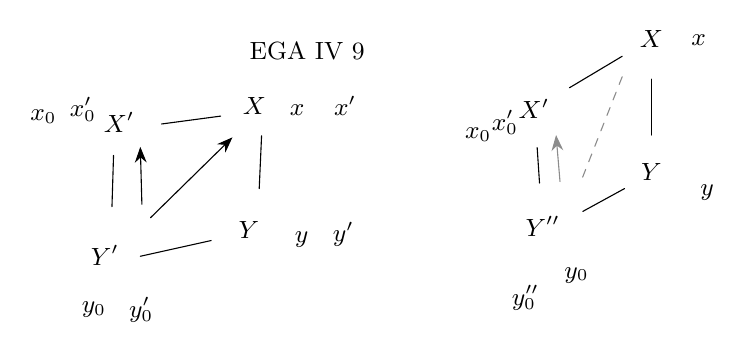
\begin{tikzpicture}[x=1mm,y=1mm,line cap=round,line join=round,font=\scriptsize]
\node[inner sep=1pt] at (22.6,-15.6) {\small $X'$};
\node[inner sep=1pt] at (39.8,-13.5) {\small $X$};
\node[inner sep=1pt] at (20.8,-32.5) {\small $Y'$};
\node[inner sep=1pt] at (39.1,-29.3) {\small $Y$};
\node[inner sep=1pt] at (13,-14.9) {\small $x_0$};
\node[inner sep=1pt] at (18,-13.9) {\small $x'_0$};
\node[inner sep=1pt] at (45.2,-14) {\small $x$};
\node[inner sep=1pt] at (51.3,-13.5) {\small $x'$};
\node[inner sep=1pt] at (45.8,-30.5) {\small $y$};
\node[inner sep=1pt] at (51.1,-29.8) {\small $y'$};
\node[inner sep=1pt] at (19.4,-39.4) {\small $y_0$};
\node[inner sep=1pt] at (25.4,-39.4) {\small $y'_0$};
\node[inner sep=1pt] at (46.5,-6.5) {\small EGA IV 9};
\draw (28,-15.8) -- (35.5,-14.8);
\draw (40.7,-17.3) -- (40.4,-24);
\draw (25.3,-32.6) -- (34.3,-30.6);
\draw (21.9,-19.8) -- (21.7,-26.3);
\draw[-{Stealth[length=2mm]}] (25.5,-26) -- (25.3,-18.7);
\draw[-{Stealth[length=2mm]}] (26.6,-27.7) -- (37,-17.5);
\node[inner sep=1pt] at (75.3,-13.9) {\small $X'$};
\node[inner sep=1pt] at (90.2,-5) {\small $X$};
\node[inner sep=1pt] at (76.4,-28.8) {\small $Y''$};
\node[inner sep=1pt] at (90.2,-21.9) {\small $Y$};
\node[inner sep=1pt] at (68.2,-17.2) {\small $x_0$};
\node[inner sep=1pt] at (71.6,-15.6) {\small $x'_0$};
\node[inner sep=1pt] at (97.3,-24.5) {\small $y$};
\node[inner sep=1pt] at (74.2,-37.9) {\small $y''_0$};
\node[inner sep=1pt] at (80.7,-35) {\small $y_0$};
\draw (79.8,-11.2) -- (86.5,-7.2);
\draw (90.2,-10.1) -- (90.2,-17.2);
\draw (81.5,-26.9) -- (86.8,-24);
\draw (75.7,-18.8) -- (76,-23.3);
\draw[-{Stealth[length=2mm]},pencil] (78.6,-23.1) -- (78.1,-17.2);
\draw[dashed,pencil] (86.5,-9.8) -- (81.3,-23);
\node[inner sep=1pt] at (96.2,-5.2) {\small $x$};
\end{tikzpicture}
\end{document}
